\clearpage
\renewcommand{\sectionprefix}{A.2}  % Set prefix for this question
\setcounter{subsection}{0}  % Reset subsection counter
\section*{Section A: Question 2}
\addcontentsline{toc}{section}{Section A: Question 2}

Comment on how the simulation time-step size impacts the numerical solution, and which method is preferred in this case.

\noindent\rule{\textwidth}{0.4pt}

\subsection{Simulation Parameters}

I implemented all three discretization methods in MATLAB with the following circuit parameters: $V_{DC} = 10$ V, $V_0 = 0$ V, $C = 1\,\mu$F, and $h = 100\,\mu$s. I also simulated the Trapezoidal method in PSCAD with chatter attenuation disabled to allow direct comparison with the analytical solution.

\subsection{Method Comparison and Selection}

\subsubsection*{Forward Euler: Rejected}

The Forward Euler method exhibits catastrophic numerical instability, as demonstrated in \Cref{fig:a02_fe_detail}. The current diverges exponentially with an amplification factor of $(R_c/R_{\epsilon})^n \approx 10^{3n}$ at step $n$ (Note that I've taken $R_\epsilon = R_c/1000$), reaching magnitudes exceeding $10^{17}$ A within microseconds. This non-physical behavior renders the method completely unsuitable for this circuit. Due to its extreme divergence, Forward Euler is shown separately and not included in the comparison plot with the other two methods.

\begin{figure}[h!]
    \centering
    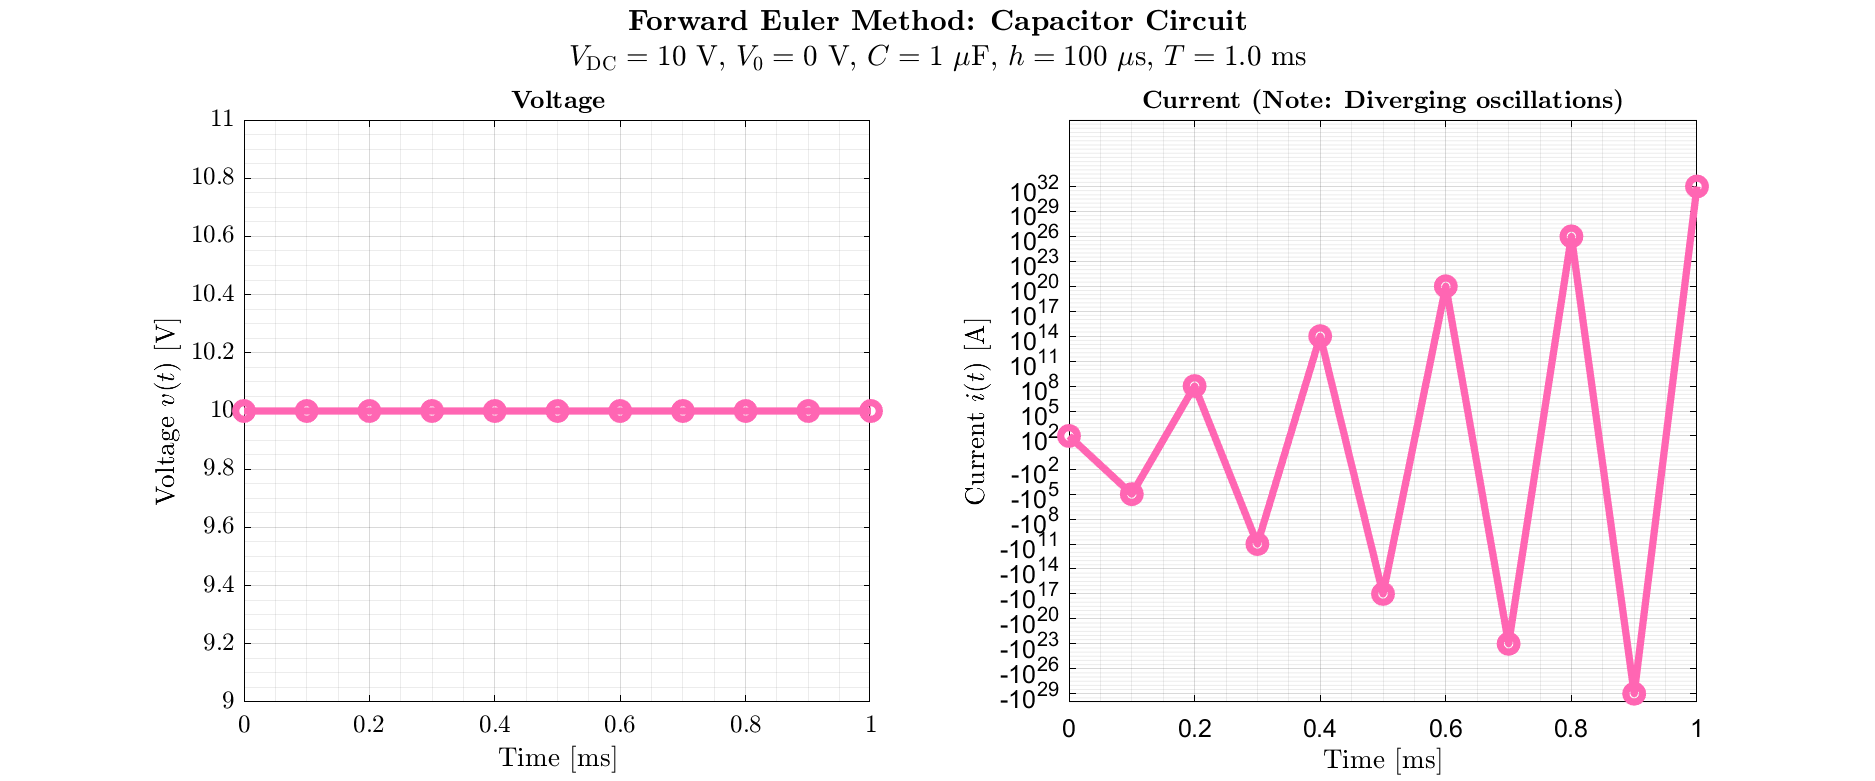
\includegraphics[width=0.85\textwidth]{figures/hw02_qA_forward-euler-method.png}
    \caption{Forward Euler method showing exponential divergence in current magnitude (symmetric logarithmic scale). The oscillations grow with successive powers of $(R_c/R_\epsilon)$, demonstrating fundamental numerical instability.}
    \label{fig:a02_fe_detail}
\end{figure}

\subsubsection*{Backward Euler vs. Trapezoidal}

\Cref{fig:a02_comparison} compares the Backward Euler and Trapezoidal methods against the PSCAD reference solution. 

\begin{figure}[h!]
    \centering
    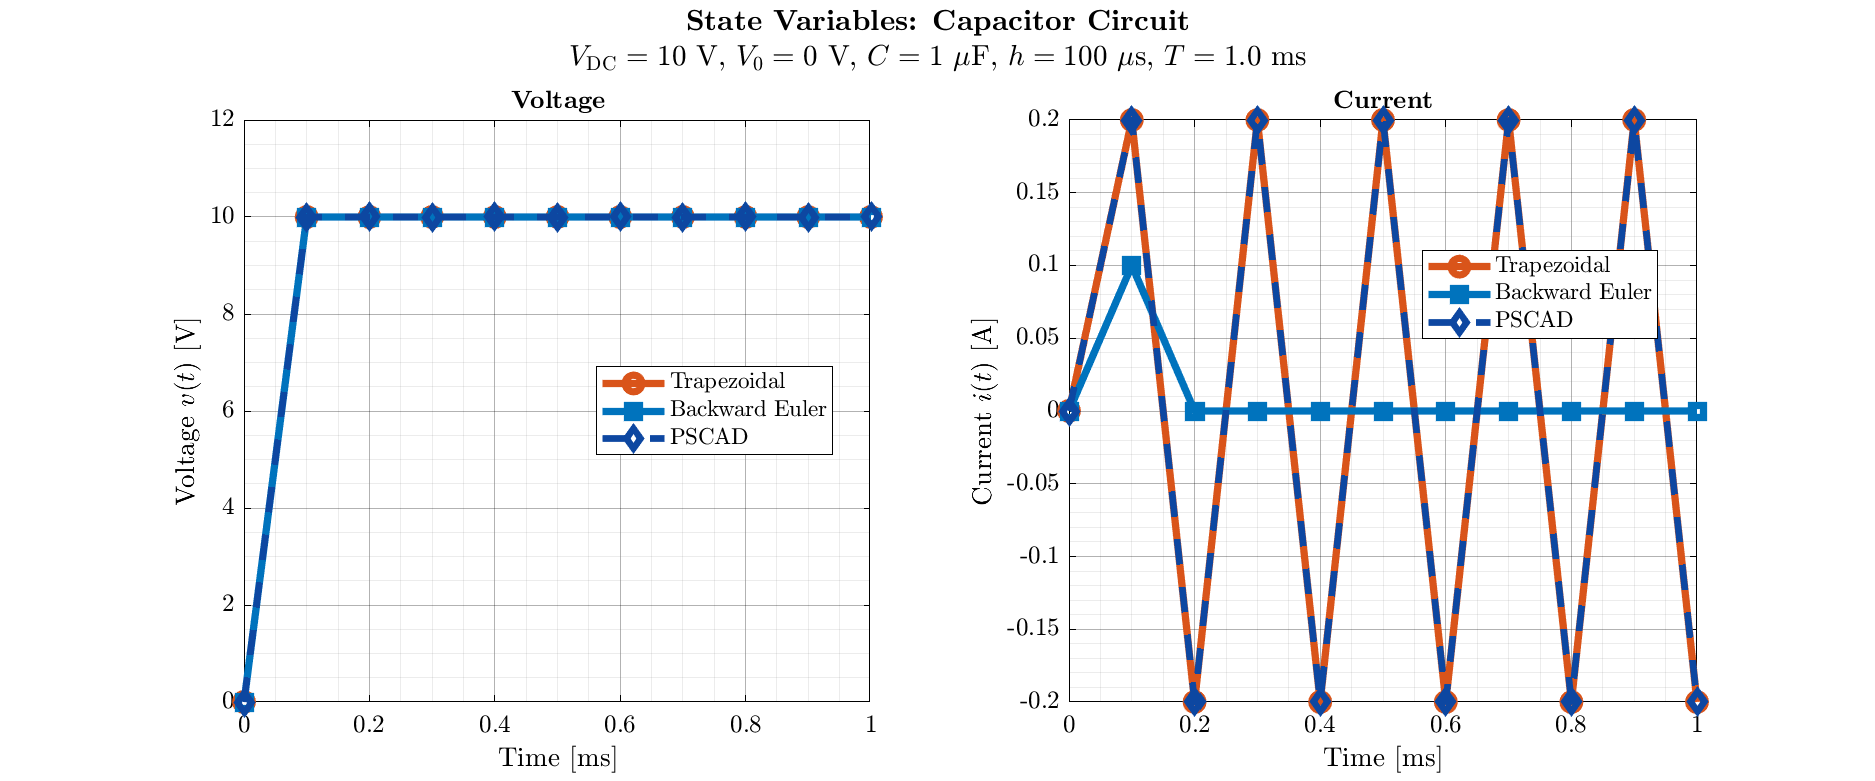
\includegraphics[width=0.85\textwidth]{figures/hw02_qA_state-variable-trajectory-comparison.png}
    \caption{Comparison of Backward Euler, Trapezoidal, and PSCAD solutions. BE provides maximum damping (minimizing current oscillations), while Trapezoidal matches PSCAD exactly and exhibits numerical chatter characteristic of lossless circuit discretization.}
    \label{fig:a02_comparison}
\end{figure}

Key observations:

\begin{itemize}
    \item \textbf{Backward Euler}: Provides maximum numerical damping, driving $i(t) \to 0$ after the initial transient. This represents the \textit{closest approach to the true steady-state solution} (zero current after capacitor charges), effectively suppressing the numerical oscillations entirely.
    
    \item \textbf{Trapezoidal}: Exhibits sustained bounded oscillations (``chatter'') due to its energy-preserving nature. My MATLAB implementation and PSCAD solution (with chatter attenuation disabled) are \textit{identical}, confirming correct implementation. The chatter is a numerical artifact of discretizing a lossless system.
    
    \item \textbf{PSCAD with chatter enabled}: When chatter attenuation is enabled in PSCAD, the solution approaches the BE behavior, demonstrating that PSCAD internally applies damping to suppress numerical oscillations.
\end{itemize}

\subsection{Impact of Step Size}

\begin{itemize}
    \item \textbf{Smaller $h$}: Reduces $R_C = h/(2C)$ for Trapezoidal, increasing chatter magnitude but maintaining stability. For BE, reduces artificial damping.
    \item \textbf{Larger $h$}: Increases numerical damping in BE (faster convergence to zero) and reduces chatter amplitude in Trapezoidal. Both remain stable.
    \item \textbf{Forward Euler}: Unstable for any step size due to the amplification factor exceeding unity.
\end{itemize}

\subsection{Preferred Method}

\textbf{Backward Euler} is preferred for this specific problem because it most closely represents the true steady-state behavior (zero current after capacitor fully charges), effectively eliminating the non-physical chatter artifacts. While Trapezoidal offers higher accuracy for transient analysis and matches PSCAD's unattenuated solution, the BE method's numerical damping produces the most physically meaningful result for a lossless capacitor reaching steady state.
